\documentclass[10pt,journal,compsoc]{IEEEtran}

\usepackage[ngerman]{babel}
\usepackage[utf8]{inputenc}
\usepackage[T1]{fontenc}
\usepackage{graphicx}
\usepackage{listings}
\usepackage[svgnames]{xcolor} % Specify colors by their 'svgnames', for a full list of all colors available see here: http://www.latextemplates.com/svgnames-colors
\usepackage[font=small,labelfont=bf]{caption} % Required for specifying captions to tables and figures

\graphicspath{{images/}}

% correct bad hyphenation here
\hyphenation{}

\begin{document}
  \title{Railway-Oriented-Programming in Clojure -- Funktionales Error-Handling}
  \author{Jan-Philipp~Willem,~Fakultät für Informatik, Hochschule Mannheim\\ 
    EFP: Entwurfsmuster für funktionale Programmierung, Sommersemster 2017
  }
  \markboth{Railway-Oriented-Programming in Clojure -- Funktionales Error-Handling}{}

  \IEEEtitleabstractindextext{%
    \begin{abstract}
Das Verhalten eines Programms nach einem Fehlerfall zu definieren, wurde bereits in vielen Programmiersprachen zu lösen versucht.
In der Praxis wird oft nur an den “Happy-Path” gedacht, oder gar gescheut den Code durch eine komplizierte Fehlerbehandlung aufzublähen.
Scott Wlaschin hat versucht den Either-Type (Monade) mithilfe des Konzepts von einzelnen Abschnitten einer Eisenbahnstrecke auf eine andere Art zu erklären und damit eine funktionale Fehler-Beachtende Herangehensweise vorgeschlagen.
Im Folgenden soll eine Umsetzung dieser Ideen in der Sprache Clojure und dessen Möglichkeiten beschrieben werden.
    % \\
    % ~\\
    % \textbf{Abstract}---
    \end{abstract}
  }
  \maketitle

  \begin{figure}[ht]
    \centering
    \vspace{-1cm}
    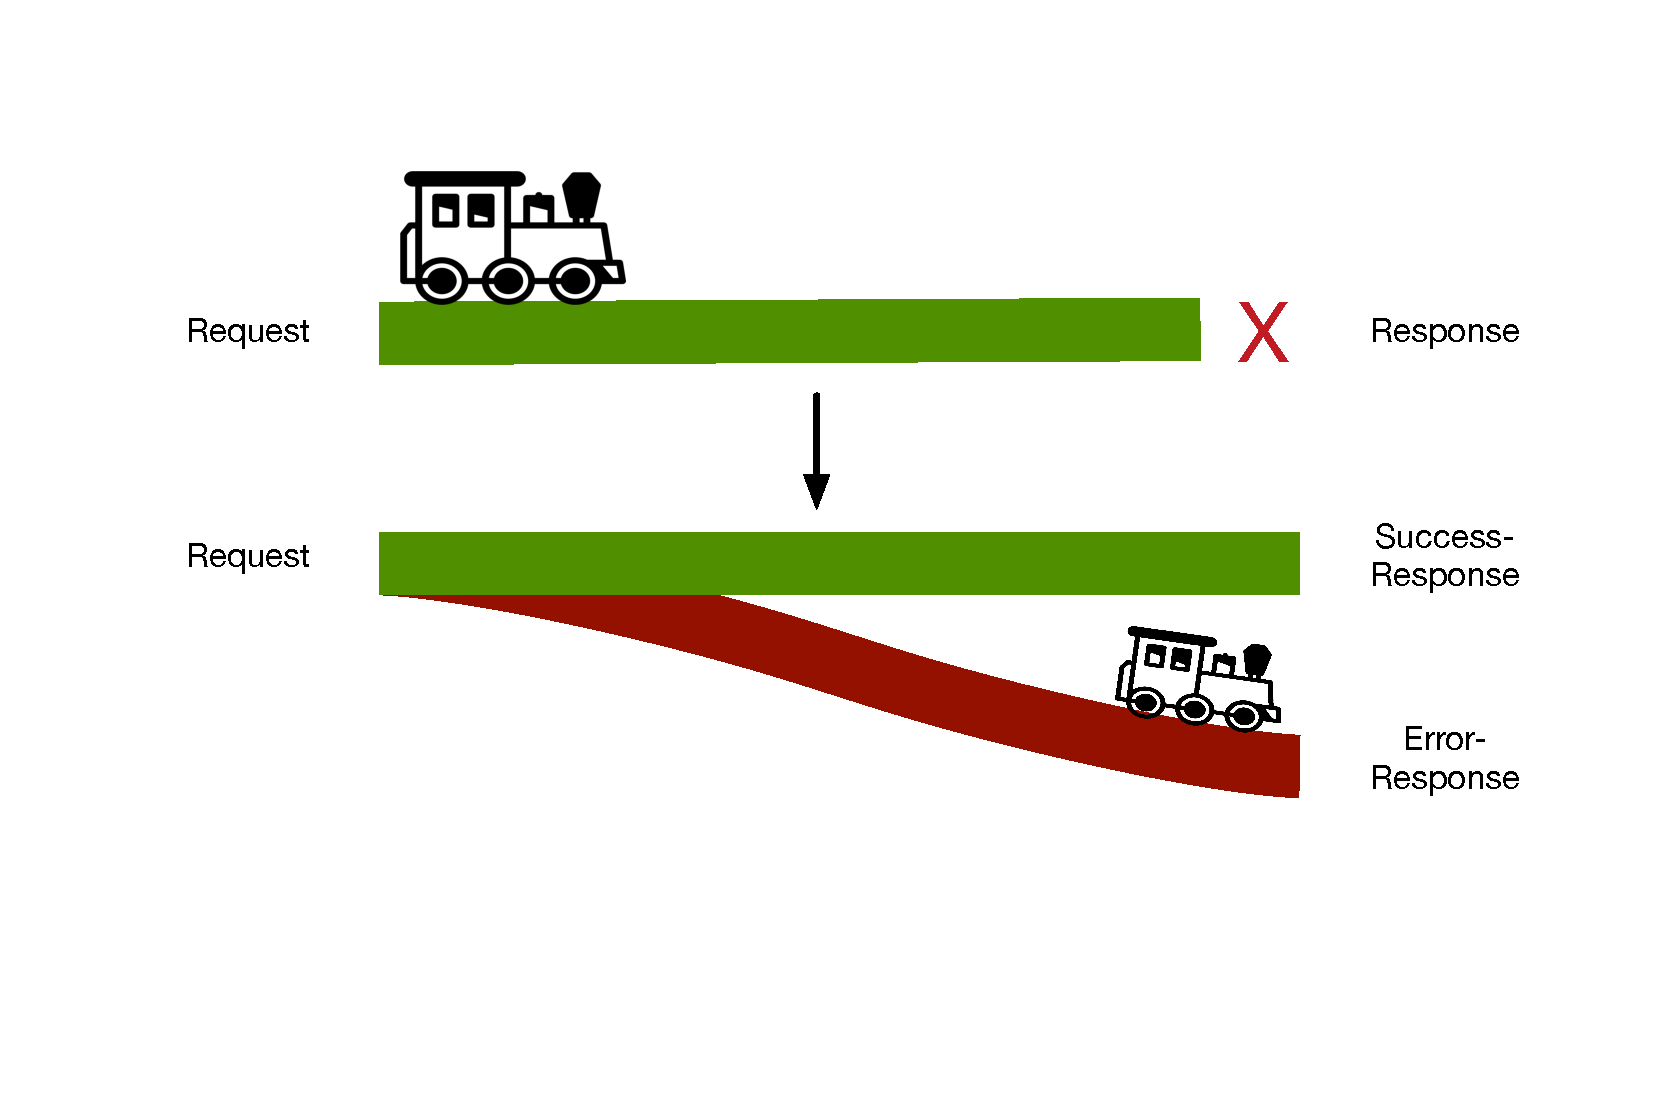
\includegraphics[width=.5\textwidth]{intro_rails_full.pdf}
    \vspace{-2cm}
    \caption{Bisherige Fehlerbehandlung und Nutzen von Zwei-Wege-Schienenteilen}\label{fig:intro}
  \vspace{.6cm}
  \end{figure}
  \IEEEraisesectionheading{
    \section{Einleitung}\label{sec:einleitung}
  }

  \IEEEPARstart{S}{cott} Wlaschin, ein bekannter F\#-Programmierer und Betreiber eines Blogs zu diesem Thema, hat ein Konzept~\cite{railwayWlaschin} vorgeschlagen um den Einstieg in eine funktionale Fehlerbehandlung bzw. ein initiales Verständnis von Monaden erheblich zu vereinfachen.
  Er nennt dies „Railway-Oriented-Programming“ (ROP) und versucht mit der Assoziation von Eisenbahn-Schienenteilen, eine Combinator-Library um den Either-Type zu gestalten.
  In seinem Vortrag über dieses Thema~\cite{railwayWlaschinNdc} möchte er klarstellen, dass er nicht der Begründer der zugrunde liegenden Theorie sei, dafür der Sache aber einen triftigen Namen geben wollte.\\
  Um diese Konzepte zu verstehen, wurden im Rahmen einer Vorlesung zu funktionalen Programmiermustern, Teile davon in der Sprache Clojure umgesetzt und auf Github~\cite{ropclojure} veröffentlicht.\\\\
  % \subsection{"`Happy-Path"'}
  Ein häufiger Fehler beim Entwickeln von Software ist die ausschließliche Betrachtung des \textbf{"`Happy-Path"'} bei einem Ausführen des Programms.
  Dies bedeutet der jeweilige Programmierer ignoriert die Existenz einer ganzen Reihe an Fehlern, welche auftreten könnten.
  Warum er so handeln sollte, könnte am Budget des jeweiligen Projekts oder aber auch an seiner Unerfahrenheit geschuldet sein.
  Allerdings ist es genauso möglich, dass bewusst gescheut wurde, den Code durch eine komplizierte Fehlerbehandlung aufzublähen.
  Das Verhalten eines Programms nach einem Fehlerfall zu definieren, ist keinesfalls einfach und wurde daher bereits in vielen Programmiersprachen zu lösen versucht.
  Merkmale einer guten Lösung, sind vor Allem ihre Wartbarkeit und in wie Weit der Code nach ihrer Integration die gleiche Eleganz aufweist, bzw. in wie Weit man die eigentliche Intention beim Lesen des Codes noch erkennen kann.\\
  Wlaschin schlägt daher vor, sich bereits bei der Architektur und dem Entwickeln Gedanken über Fehler und ihre Implikationen zu machen. Er nennt dies \textbf{"`Error-by-design"'}, indem man Fehlermeldungen als integraler Bestandteil der Applikation bzw. von ihren Funktionen macht.
  % \subsection{"`Error-by-design"'}

  \section{Railway-Oriented-Programming}
  Es sollen zunächst folgende grundlegende Schienen-Teile betrachtet werden:
  \begin{itemize}
    \item Result: Success/Failure
    \item switch
    \item switch-functions
    \item bind/bind-pipe
    \item switch-compose
  \end{itemize}
  Die Grundüberlegung besteht in der Erwartung, dass eine Funktion von nun an nicht nur einen einzigen Rückgabewert besitzt.
  Es soll zwischen einem gutartigen Ergebnis (\textbf{Success}) und einem Fehlerfall (\textbf{Failure}) unterschieden werden können.
  Dies ist durch ein Leichtes erzielbar, indem man einen \textbf{Result}-Typ definiert, welcher als Envelope das eigentliche Ergebnis einer Funktion oder eine jeweilige Fehlermeldung enthält.\\
  Eine Funktion die unseren Result-Typ nutzt, soll im Weiteren als eine \textbf{switch-function} bezeichnet werden, da sie wie eine Weiche in der Bahnfahrt reagiert, welche bei einem Fehler den Datenfluss von dem Success-Path auf den Failure-Path leitet.
  Abbildung~\ref{fig:intro} versucht dieses Verhalten zu visualisieren.
  Ein typisches Beispiel für so eine Funktion wäre eine spezifische Form-Feld-Validierung, welche jeweilig als einzelnen Schritt in unserem ROP-Datenfluss dargestellt werden kann.\\
  Um eine bereits bestehende Funktion unverändert zu integrieren, kann sie mit \textbf{switch} mit einer Funktions-Komposition vereint werden, womit ihr eigentliches Ergebnis in ein Success konvertiert wird.\\
  Um zwei switch-functions miteinander zu verbinden, wird die Funktion \textbf{bind} genutzt, welche die Success- und Failure-Paths miteinander verbindet.
  Da die Sprache Clojure ein Lisp-Dialekt ist, liegt es nahe, bind auch für die Übergabe einer Liste mit mehreren switch-functions zu definieren.
  So führt \textbf{bind-pipe} (\texttt{>>=}) eine beliebige Anzahl an Forms nacheinander aus und leitet jeweils den Result-Typ der nächsten Funktion als letzten Parameter zu.
  Es entsteht ein in sich geschlossenes Zwei-Wege-Schienensystem.
  In Abbildung~\ref{fig:bind} werden die Schienenteile bind und bind-pipe dargestellt.
  Dabei fühlt sich die Vorgehensweise an, als ob man das thread-first macro (\texttt{->}) genutzt hätte, welches man in anderen Sprachen auch als pipe oder left-to-right-composition bezeichnet.\\
  Mit \textbf{switch-compose} kann man switch-functions im Vergleich zu bind auf eine andere Art miteinander verbinden.
  Es kann so aus jeweils zwei switch-functions eine Komposition gebildet werden, welche sich benutzen lässt, als wäre es eine einzige Funktion. (siehe Abbildung~\ref{fig:compose})
  Es kann so ein ganzer Baum (Abb.~\ref{fig:compose_recursive}) an verschachtelten switch-functions entstehen.
  Je nach Use-Case bietet sich eher der Einsatz von bind oder switch-compose an.\\
  Die Implementierung der beschrieben Funktionen kann auf Github~\cite{ropclojure} betrachtet werden.
  Hilfreich zum Verständnis sind dabei auch ihre jeweiligen Tests.
  Ziel soll es noch werden, die Funktionen als Makros zu definieren.
  Bisherig wurden Funktionen aus dem clojure.core und der Pattern-Matching Funktion core.match~\cite{corematch} genutzt.
  Weiterhin war die Clojure Sequence-Abstraction und Rest-Parameters sehr hilfreich.

  \begin{figure}[h]
    \centering
    \vspace{-.5cm}
    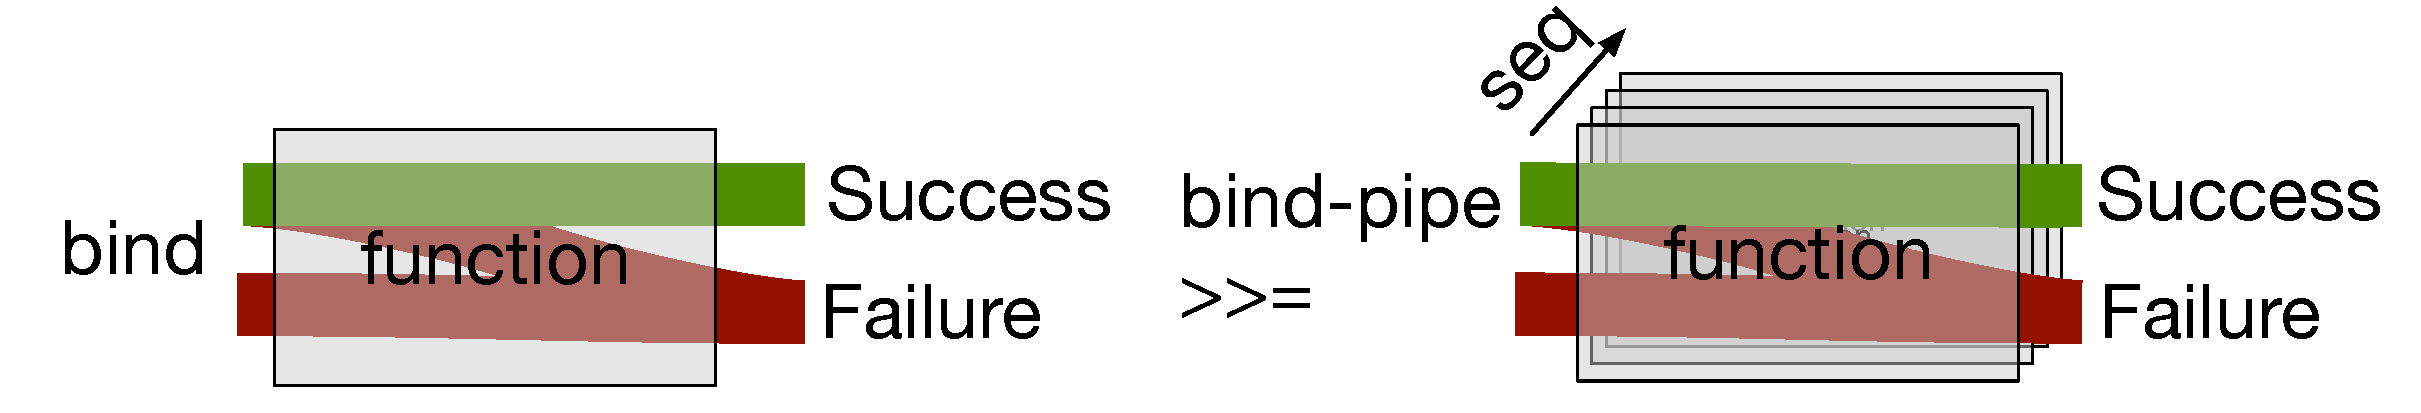
\includegraphics[width=.5\textwidth]{bind_figure.pdf}
    % \vspace{-2cm}
    \caption{bind und bind-pipe}\label{fig:bind}
  % \vspace{.3cm}
  \end{figure}
  \begin{figure}[h]
    \centering
    \vspace{-.3cm}
    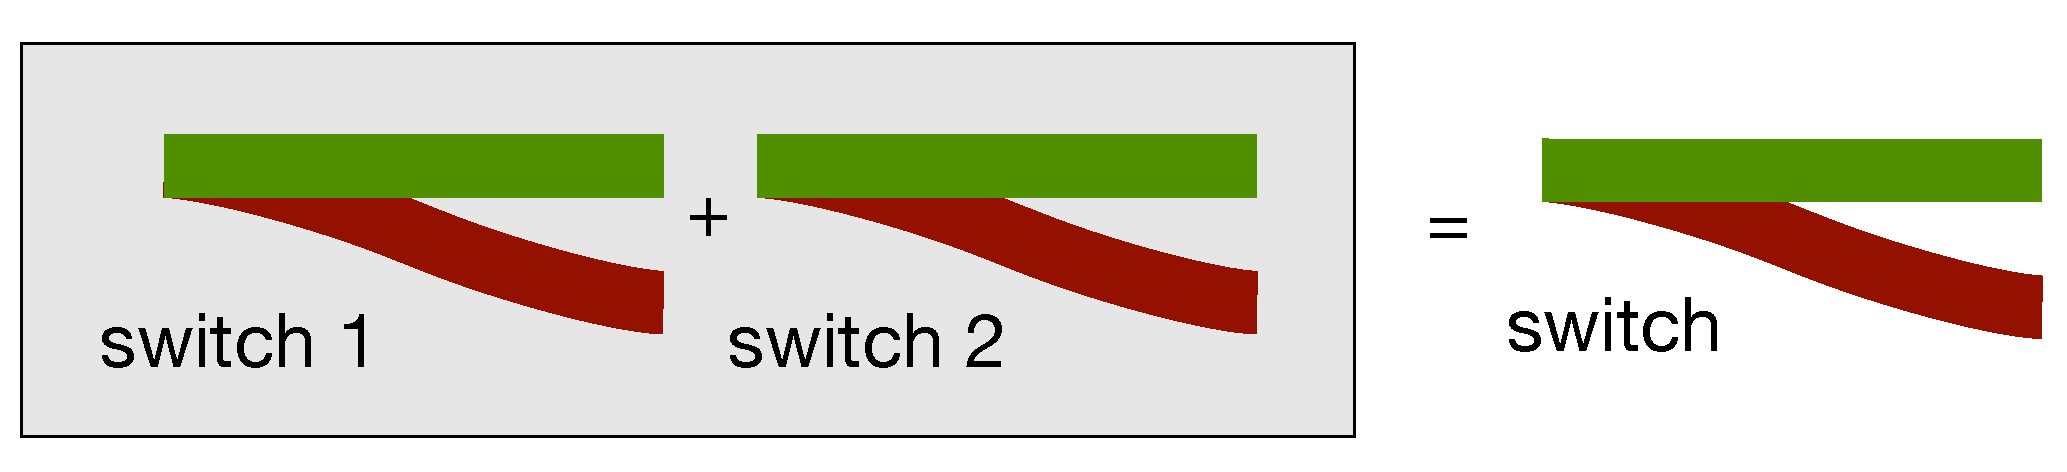
\includegraphics[width=.5\textwidth]{compose_figure.pdf}
    % \vspace{-2cm}
    \caption{switch-compose resultiert in einzelne switch-function}\label{fig:compose}
  % \vspace{.6cm}
  \end{figure}
  \begin{figure}
    \centering
    % \vspace{-.3cm}
    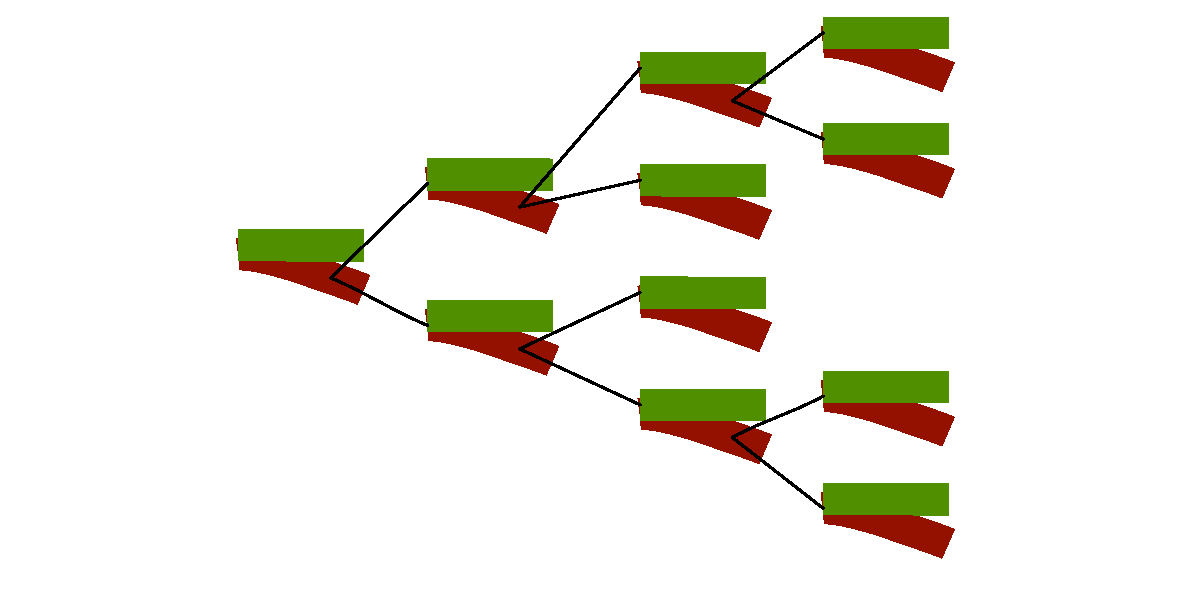
\includegraphics[width=.5\textwidth]{compose_recursive.pdf}
    % \vspace{-2cm}
    \caption{Ein Baum von verschachtelten switch-functions}\label{fig:compose_recursive}
  % \vspace{.6cm}
  \end{figure}
  \subsection{Weitere Schienenteile}
  In Erweiterung zu den Grundlegenden Schienenteilen sind weitere folgende denkbar:
  \begin{itemize}
    \item try/catch
    \item log/tee
    \item map-parallel
    % \item ..
  \end{itemize}
  Viele bisherige Implementierungen, welche man verwenden möchte, beruhen auf der Fehlerbehandlung von \textbf{try/catch}, beziehungsweise auf Exceptions.
  Um diese jeweiligen Funktionen in ein Zwei-Wege-System zu integrieren, kann man wiederum eine Hilfsfunktion bauen.\\
  Seiteneffekte wie \textbf{logging} oder beliebige Andere wie eine Persistenz in einer Datenbank (vergl. cli-tool \textbf{tee}), können mit der gleichen Vorgehensweise genutzt werden.
  Entscheidend dabei ist, dass die Seiteneffekte keine Änderungen an dem Ergebnis des Datenflusses machen, sondern nur externe Ereignisse auslösen.
  Wlaschin bezeichnet diese Funktionen auch als Dead-End-Functions, weil ihr Schienenteil ein Enstück darstellt.\\
  Um mehrere Ergebnisse von switch-functions zu evaluieren, ohne bei einem Fehler sofort abzubrechen, bietet sich ein \textbf{map-parallel} an.
  Solch ein Verhalten möchte man beispielsweise bei einer Formular-Validierung erhalten, welche mehrere Funktionen pro Feld nutzt.

  \section{Fazit}
  Abschließend ist zu sagen, dass das Konzept der Fehlerbehandlung über einen Result-Typ und dessen dazugehörigen Hilfsfunktionen am Anfang im Vergleich zu dem bisherigen Weg sehr kompliziert wirkt.
  Weiterhin ist bei der Arbeit mit einem Team darauf zu achten, dass alle Entwickler neue Funktionen in den ROP-Datenfluss integrieren sollten.
  Bei einer konsistenten Anwendung, kann es im Gegenzug wirklich hilfreich sein, da man nun nicht mehr raten muss, ob eine Funktion bei einem Fehler nun nichts tut, Null oder bspw. einen negativen Wert zurückgibt.
  Man erhält so eine stabile und leicht wartbare Basis für eigene Implementierungen.\\
  Als ein gutes Beispiel für konsistente Fehlerbehandlung, sind die Grund-Funktionen von Elm~\cite{elm} zu betrachten, welche grundsätzlich alle, bei kritischen Stellen, eine Result- oder Maybe-Monade für den Rückgabewert nutzen.\\
  Gegen Ende des Projektes wurde der Schreiber dieser Arbeit auf zwei weitere interessante Umsetzungen von ROP in Clojure aufmerksam. \cite{otherrop} bedient sich einer Clojure-Library~\cite{clojurecats}, welche Konzepte der Kategorie-Theorie umsetzt.
  Und eine weitere Implementierung~\cite{otherrop2}, ist bereits als Paket in Leiningen verfügbar.

  \begin{thebibliography}{1}
    \bibitem{railwayWlaschin}
      Scott Wlaschin, \emph{Railway-Oriented-Programming -- a functional approach to error handling}, https://fsharpforfunandprofit.com/rop/
    \bibitem{railwayWlaschinNdc}
      Scott Wlaschin, \emph{NDC Conference 2014},\\https://vimeo.com/113707214
    \bibitem{ropclojure}
    J. Willem \emph{ROP in Clojure},\\https://github.com/jwillem/rop-clojure
    \bibitem{clojurebook}
    D. Higginbotham, \emph{Clojure for the Brave and True},\\https://braveclojure.com
    \bibitem{otherrop}
      ah45, \emph{railway oriented programming},\\https://gist.github.com/ah45/7518292c620679c460557a7038751d6d
    \bibitem{corematch}
      Clojure Core Team, \emph{Core.match -- a Pattern Matching Function}, https://github.com/clojure/core.match/wiki/Basic-usage
    \bibitem{otherrop2}
    HughPowell, \emph{railway-oriented-programming},\\
    https://github.com/HughPowell/railway-oriented-programming
    \bibitem{clojurecats}
      Funcool, \emph{Cats -- Category Theory and Algebraic abstractions in Clojure}, https://github.com/funcool/cats
    \bibitem{elm}
      Elm, \emph{Gut gelößtes Sprachkonzept mit Maybe \& Either in Elm}, https://guide.elm-lang.org/error\_handling
  \end{thebibliography}
  Die Links wurden zuletzt am 07.07.2017 besucht.
\end{document}
